\subsection{Product perspective} 
The product we will provide is an application distributed for any kind of device that supports Android as operative system. This application will immediately be useble as soon as you install it on a device.
It will not have any internal interface for administration but it will be only user based.

\begin{figure}[!h]
	\centering
	\makebox[\textwidth][c]{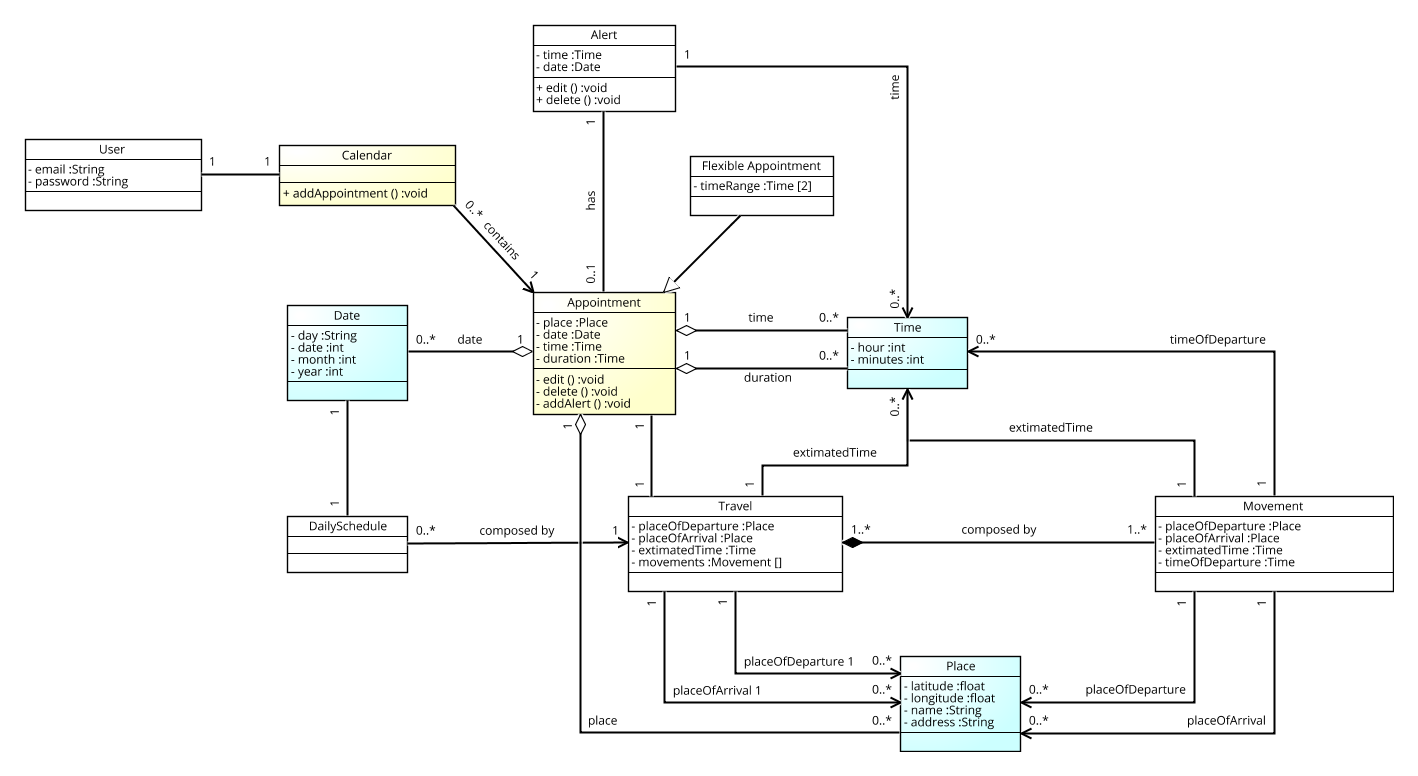
\includegraphics[width=1.2\textwidth]{Images/ClassDiagram.png}}%
\end{figure}

(UML e stateCharts)

\subsection{Product functions}
This application aims to provide a smart calendar, which schedules the best organization, taking account of your personal appointments, which you inserted in the calendar. The computed schedule depends on some preferences that you filled out and you can modify them when you want.
\subsection{User characteristics}
We recommend the application to a person who wants to organize easily his time in the best way. He will be able to benefit from this service in a very simple way because Travlendar+ requires only basic knowledge of a simple calendar. After registering an account, the application is ready to handle his commitments, so scheduling the best organization.
\subsection{Domain Assumption and Dependencies}
\begin{itemize}
	\item For any day user can create unlimited number of events.
	\item User has only one calendar.
	\item There isn’t any dependence between users.
	\item User can choose among some alternative travel proposals.
	\item If an event is overlapping another one, the user must select a choice from the choices proposed.
	\item User can delete an event.
	\item User can modify an event already created.
	\item User can change the scheduling proposed.
	\item User can select in which preferences the scheduling based on.
	\item Notification of best proposal will be shown.
	\item Notification of any problem that occurs will be shown.
\end{itemize}
\subsection{Constrains}
Travlender+ requires:
\begin{itemize}
	\item Internet connection enabled on own device
	\item GPS available on own device
	\item Login during the first access
	\item Initially registration with an account
	\item Android device
	\item Milano as the default city
	\item 30 Mb(?) of storage memory available on own devise to be installed
\end{itemize}


